\chapter{深度生成式建模}\label{ch:overview-dgm}

\epigraph{
    \textit{我所不能创造的，我就不能理解。}}{Richard P. Feynman}

% \ys{This might be a good place to quote Richard Feynmann on ``What I cannot create, I do not understand.''}

% \jcc{need to rewrite the following: 
% At the heart of deep generative modeling (DGMs) is a compelling goal: teaching machines to create. Picture a system that studies thousands of images, musical pieces, or artworks—and then conjures something entirely new, yet strikingly faithful to the style and structure of its inspirations. This is more than copying; it is a learned capacity to generate original content grounded in the patterns of real-world data.}

% Deep generative models (DGMs) aim to approximate the complex and high dimensional probability distributions underlying real world data. Through unsupervised learning, they acquire the ability to synthesize novel artifacts such as images, text, video, or audio that are statistically consistent with the learned distribution.
% \se{this paragraph could be made more precise and clear}

深度生成模型（DGM）是学习高维数据（如图像、文本、音频）上概率分布的神经网络，从而能够生成与数据集相似的新样本。我们用 $p_{\bphi}$ 表示模型分布，用 $p_{\mathrm{data}}$ 表示数据分布。给定一个有限的数据集，我们通过最小化衡量 $p_{\bphi}$ 与 $p_{\mathrm{data}}$ 之间差距的损失来拟合 $\bphi$。训练完成后，生成即运行模型的采样过程以抽取 $\rvx \sim p_{\bphi}$（密度 $p_{\bphi}(\rvx)$ 能否直接计算取决于模型类别）。模型质量由生成的样本及其汇总统计量与 $p_{\mathrm{data}}$ 的匹配程度，连同任务特定或感知度量来评判。


本章构建了这些思想背后的数学与概念基础。我们在 \Cref{sec:formulation-dgm} 中形式化该问题，在 \Cref{sec:examples-dgm} 中介绍代表性的模型类别，并在 \Cref{sec:taxonomy} 中总结实用的分类体系。








% \ys{This type of motivating language is crucial to the success of the monograph, but it currently lacks the depth and force that a compelling vision should convey. I'd like to try rewriting all such paragraphs once we've addressed all the other issues.}
% \jcc{I rewrote it as the above brown part.}


% To understand how this creative synthesis becomes feasible, this chapter establishes the mathematical and conceptual foundations of modern generative models.

% We begin by formalizing the core problem in \Cref{sec:formulation-dgm}, introducing the key mathematical tools and notation that drive this field. While a diverse array of DGMs exists, as overviewed in \Cref{sec:examples-dgm}, our focus will narrow to three prominent classes of DGMs that are closely connected to diffusion models. These are: Variational Autoencoders (VAEs), which we discuss in \Cref{sec:vae}; Energy-Based Models (EBMs), introduced in \Cref{sec:ebm}; and Normalizing Flows (NFs), explored in \Cref{sec:flow-based-method}.  Through this exploration, readers will gain a comprehensive understanding of the principled foundations that underpin modern diffusion-based generative modeling, as developed in subsequent chapters.


\newpage
\section{什么是深度生成式建模？}\label{sec:formulation-dgm}

% \se{i feel a more algorithmic description describing the inputs (data) and the output (trained network) is the right level of abstraction to start}



DGM 以从未知且复杂的分布 $p_{\mathrm{data}}$ 中抽取的大量真实世界样本
（如图像、文本）作为输入，
输出一个参数化近似分布 $p_{\bphi}$ 的、已训练好的神经网络。其目标有两方面：
\begin{enumerate}
\item \textbfs{逼真生成：}生成与真实数据无法区分的、新颖逼真的样本。
\item \textbfs{可控生成：}实现对生成过程的细粒度、可解释的控制。
\end{enumerate}



% \ys{The words ``mimicry'' and ``mastery'' are unnecessarily obscure in this context.} \jcc{revised!}

% The capabilities of DGMs extend far beyond data synthesis. They have emerged as foundational tools across a wide range of domains: from restoring corrupted data and intelligently filling in missing information (inpainting) to simulating complex phenomena and driving new forms of creative content generation. \se{a bit odd to have this text here, isn't it contrallable generation?}

本节介绍 DGM 背后的基本概念与动机，为后续详细探讨其数学框架与实际应用做准备。


\subsection{数学设定}\label{subsec:intro-math-setup}
我们假设可以获得从潜在的复杂数据分布 $ p_{\mathrm{data}}(\mathbf{x}) $ 中独立同分布（i.i.d.）抽取的一组有限样本\footnote{这是机器学习中的常见假设。为简便起见，我们用符号 $ p $ 同时表示概率分布或其概率密度/质量函数，视上下文而定。}。


\paragraph{DGM 的目标。}

DGM 的首要目标是从有限数据集中学习一个可处理的概率分布。这些数据点是假设从未知且复杂的真实分布 $p_{\mathrm{data}}(\rvx)$ 中采样得到的观测值。由于 $p_{\mathrm{data}}(\rvx)$ 的形式未知，我们无法直接从中抽取新样本。因此，核心挑战在于构建一个能够充分近似该分布的模型，以实现新逼真样本的生成。

为此，DGM 使用深度神经网络来参数化模型分布 $p_{\bm{\phi}}(\rvx)$，其中 $\bm{\phi}$ 表示网络的可训练参数。训练目标是找到最优参数 $\bm{\phi}^\ast$，使模型分布 $p_{\bm{\phi}}(\rvx)$ 与真实数据分布 $p_{\mathrm{data}}(\rvx)$ 之间的散度最小。从概念上讲，
\[
p_{{\bm{\phi}}^\ast}(\rvx) \approx p_{\mathrm{data}}(\rvx).
\]




% The primary objective of deep generative modeling (DGM) is to learn \se{learn what?} from a finite dataset sampled from an unknown true distribution $p_{\mathrm{data}}(\mathbf{x})$, and to generate new samples that closely resemble this data. Since the explicit form of $p_{\mathrm{data}}(\mathbf{x})$ is unknown, the core challenge lies in approximating and efficiently sampling from this complex distribution \se{confusing, we never sample from pdata, only pmodel} to enable realistic and data-consistent generation based on limited observations.


% To this end, we use a deep neural network to construct a parametrized model density $p_{\bm{\phi}}(\rvx)$, where ${\bm{\phi}} \in \Phi$ denotes the model parameters \se{model and network terminology creates unnecessary ambiguity} and $\Phi$ represents the set of all possible parameter values. The objective is to find the optimal parameters ${\bm{\phi}}^\ast \in \Phi$ such that  
% \[
% p_{{\bm{\phi}}^\ast}(\rvx) \approx p_{\mathrm{data}}(\rvx).
% \]
% \se{i would rephrase slightly to avoid the potential confusion that networks have finite capacity so the above is not possible}

当统计模型 $p_{{\bm{\phi}}^\ast}(\rvx)$ 充分逼近数据分布 $p_{\mathrm{data}}(\rvx)$ 时，它可以作为生成新样本和评估概率值的代理。这一模型 $p_{\bm{\phi}}(\rvx)$ 通常被称为\emph{生成模型}。


\paragraph{DGM 的能力。}
一旦有了数据分布的代理 $p_{\bm{\phi}}(\rvx)$，我们就可以使用诸如从 $p_{\bm{\phi}}(\rvx)$ 中进行蒙特卡洛采样等采样方法，生成任意数量的新数据点。此外，对于任意给定样本 $\rvx'$，我们可以评估模型密度 $p_{\bm{\phi}}(\rvx')$，这通常被非正式地称为模型赋予 $\rvx'$ 的“似然”\footnote{严格来说，对于连续数据，$p_{\bm{\phi}}(\rvx')$ 是在 $\rvx'$ 处求值的密度，而非观测到该精确样本的概率。我们遵循机器学习领域的惯常简写，将该量称为样本的“似然”。}。

\begin{figure}
\vspace{-0.5cm}
    \centering
    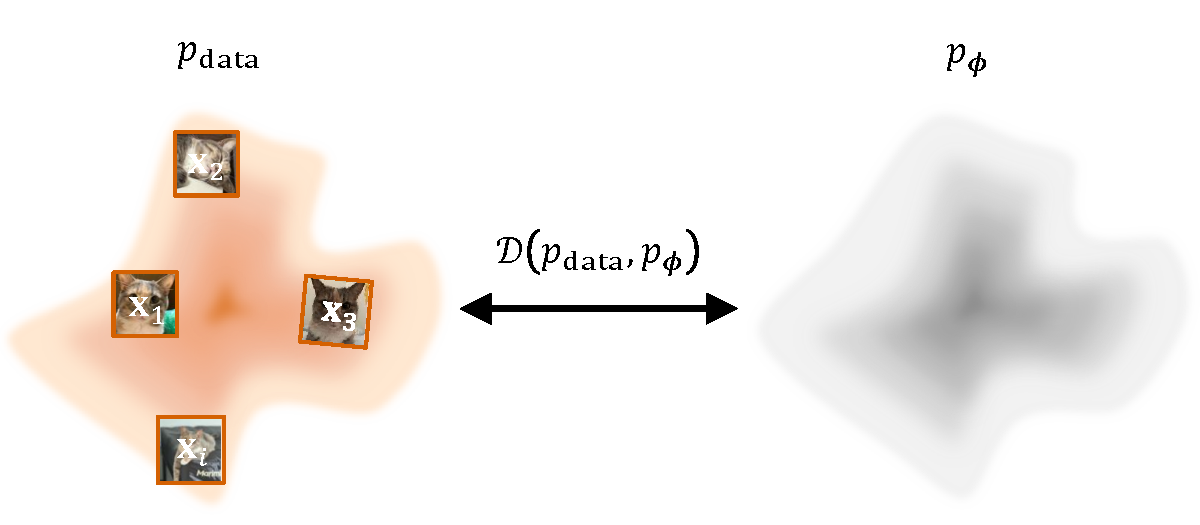
\includegraphics[width=0.9\linewidth]{Images/PartB/dgm-learning.pdf}
    \vspace{-0.2cm}
    \caption{\textbfs{DGM 目标示意图。}训练 DGM 本质上是最小化模型分布 $p_{\bm{\phi}}$ 与未知数据分布 $p_{\mathrm{data}}$ 之间的差异。由于 $p_{\mathrm{data}}$ 无法直接访问，这一差异必须利用从中抽取的有限独立同分布（i.i.d.）样本 $\rvx_i$ 来高效估计。\figcredit{由作者绘制。}}
    \label{fig:dgm-training}
\end{figure}

% \paragraph{Training of DGM.}
% To train the model, we define a discrepancy measure $\mathcal{D}(\cdot, \cdot)$ that quantifies the difference between the data distribution $p_{\mathrm{data}}$ and the model distribution $p_{\bm{\phi}}$. Since the true data distribution is unknown, this discrepancy must be estimated efficiently using a finite set of independent and identically distributed (i.i.d.) samples drawn from $p_{\mathrm{data}}$. The optimal parameter $\bm{\phi}^\ast$ is then obtained by solving the following optimization problem based on this empirical estimate:
% \begin{align}\label{eq:dgm-optimization}
%     \bm{\phi}^\ast = \arg\min_{\bm{\phi} \in \Phi} \mathcal{D}(p_{\mathrm{data}}, p_{\bm{\phi}}).
% \end{align}
% If the parameter space $\Phi$ is sufficiently large and the model family $\{p_{\bm{\phi}}\}_{\bm{\phi} \in \Phi}$ is expressive enough, then $p_{\bm{\phi}^\ast}(\mathbf{x})$ can closely approximate $p_{\mathrm{data}}(\mathbf{x})$.


% \ys{One missing factor is there must exist an efficient way to estimate this discrepancy measure using iid samples from the data distribution.}

% There are various choices for the discrepancy measure $\mathcal{D}$~\citep{cover1999elements}, including the Wasserstein distance, total variation distance, Jensen–Shannon divergence, Fisher divergence (spoiler: notably related to diffusion models), and the Kullback–Leibler (KL) divergence. Each induces a different training objective, with distinct trade-offs in sensitivity, smoothness, and optimization dynamics. Among them, the KL divergence is especially popular due to its close connection to maximum likelihood estimation, as discussed next.
% \se{instead of throwing all this jargon at the reader, i would start with an example (KL) and then tell them there are other options}

% \subparagraph{Kullback-Leibler Divergence.}
% \jc{
% A widely used choice for $\mathcal{D}$ is the Kullback–Leibler (KL) divergence, denoted by $\mathcal{D}_{\mathrm{KL}}(\cdot \| \cdot)$, which measures the discrepancy between the data distribution $p_{\mathrm{data}}$ and the model distribution $p_{\bm{\phi}}$. It is defined as
% \begin{align*}
%     \mathcal{D}_{\mathrm{KL}}(p_{\mathrm{data}} \| p_{\bm{\phi}}) 
%     &:= \int p_{\mathrm{data}}(\mathbf{x}) \log \frac{p_{\mathrm{data}}(\mathbf{x})}{p_{\bm{\phi}}(\mathbf{x})} \, \diff \mathbf{x} \\
%     &= \mathbb{E}_{p_{\mathrm{data}}} \left[ \log \frac{p_{\mathrm{data}}(\mathbf{x})}{p_{\bm{\phi}}(\mathbf{x})} \right],
% \end{align*}
% where the integral is a Lebesgue integral\footnote{Throuout the monograph, if without stating, the integration of deterministic mappings is understood as Lebesgue sense.}, which reduces to a summation when the distributions are defined over discrete spaces.

% The KL divergence is asymmetric, i.e., 
% \[
% \mathcal{D}_{\mathrm{KL}}(p_{\mathrm{data}} \| p_{\bm{\phi}}) \neq \mathcal{D}_{\mathrm{KL}}(p_{\bm{\phi}} \| p_{\mathrm{data}}).
% \]Importantly, minimizing $\mathcal{D}_{\mathrm{KL}}(p_{\mathrm{data}} \| p_{\bm{\phi}})$ encourages \emph{mode covering}: the model is penalized heavily if it assigns low probability to regions where the data density is high. This pushes the model to cover all modes of the data distribution, avoiding mode collapse.
% }
% \se{add an extra sentence actually showing it using the formula, e.g. if pmodel is zero when pdata is not}

% \ys{It may be useful to note somewhere that the integrals below refer to Lebesgue integrals, which reduce to summations when defined over counting measures.}

% \ys{No need to expand so much on the following list. Just mention it has the ``mode covering'' property, and explain what it means and why in a few sentences (ChatGPT can do this).} \jcc{Revised!}

% \se{important to note somewhere that pdata can't be evaluated, which is a good motivation for the MLE stuff below}

% Crucially, it is equivalent to \emph{Maximum Likelihood Estimation} (MLE), as detailed below.
% \subparagraph{Maximum Likelihood Training.}
% From the definition of $\mathcal{D}_{\mathrm{KL}}$, we derive:
% \begin{align*}
%     \mathcal{D}_{\mathrm{KL}}(p_{\mathrm{data}} \| p_{\bm{\phi}}) 
%     &= \displaystyle\int  \log \frac{p_{\mathrm{data}}(\mathbf{x})}{p_{\bm{\phi}}(\mathbf{x})} p_{\mathrm{data}}(\mathbf{x}) \diff \rvx \\
%     &= -\mathbb{E}_{\rvx \sim p_{\mathrm{data}}} \left[ \log p_{\bm{\phi}}(\mathbf{x}) \right] + C,
% \end{align*}
% where $C := \mathbb{E}_{\rvx \sim p_{\mathrm{data}}} \left[\log p_{\mathrm{data}}(\mathbf{x})\right]$ is constant with respect to $\bm{\phi}$. Hence, minimizing KL divergence is equivalent to maximizing the log-likelihood: 
% % \ys{``Message'' feels weird in this context. Maybe better to call it ``remark'', or ``observation''?}
% \msg{Observation}{Minimizing KL $\Leftrightarrow$ Maximum Likelihood Estimation}{
% \begin{align}\label{eq:MLE}
%     \min_{\bm{\phi}} \mathcal{D}_{\mathrm{KL}}(p_{\mathrm{data}} \| p_{\bm{\phi}}) \Longleftrightarrow \max_{\bm{\phi}}\mathbb{E}_{\rvx\sim p_{\mathrm{data}}}\left[\log p_{\bm{\phi}}(\rvx)\right].
% \end{align}
% }
% MLE is a classical method for learning probabilistic models by finding parameters $\bm{\phi}$ that maximize the likelihood of the observed data, rather than explicitly reconstructing the data points. \se{maybe move after you introduce the empirical (not population) version, otherwise there is no observation/data}

% To implement MLE in practice, we often minimize the KL divergence between the data and model distributions, approximated using a finite set of training samples  $\{\mathbf{x}^{(i)}\}_{i=1}^N$:
% \begin{align*}
%     \mathcal{D}_{\mathrm{KL}}(p_{\mathrm{data}} \| p_{\bm{\phi}}) 
%     &\approx  -\frac{1}{N} \sum_{i=1}^N \log p_{\bm{\phi}}(\mathbf{x}^{(i)}) + C,
% \end{align*}
% with $C = \frac{1}{N} \sum_{i=1}^N \log p_{\mathrm{data}}(\mathbf{x}^{(i)})$.
% \se{this is strange and potentially confusing, i would avoid the C estimate part since that is not something we can do "in practice"}


% \jc{While the model could theoretically assign arbitrarily high density to training points (a countable set with measure zero), in practice, neural networks avoid forming delta distributions due to their continuous and smooth architectures, finite capacity, and regularization (e.g., weight decay, dropout), which prevent overfitting.} \ys{I think you're confusing density functions with mass functions here. For continuous distributions, the optimal model distribution is indeed a delta distribution. The model's density function can take arbitrarily high values at data points, since these are countable. The integral of a probability density function is unaffected by its values on a countable set. The fact that our model distributions do not collapse to delta distributions cannot be attributed to the normalization constraint.} \jcc{Revised!}
% \se{not sure why overfitting/regularization is relevant here; it's not particularly specific to the loss used to train generative models}


\paragraph{DGM 的训练。}
我们通过最小化差异 $\mathcal{D}(p_{\mathrm{data}},p_{\bm{\phi}})$ 来学习模型族 $\{p_{\bm{\phi}}\}$ 的参数 $\bm{\phi}$：
\begin{align}\label{eq:dgm-optimization}
  \bm{\phi}^\ast \in \arg\min_{\bm{\phi}}\; \mathcal{D}(p_{\mathrm{data}},p_{\bm{\phi}}).
\end{align}
由于 $p_{\mathrm{data}}$ 未知，$\mathcal{D}$ 的实际选择必须能够基于来自 $ p_{\mathrm{data}} $ 的独立同分布样本进行高效估计。
在容量充足时，$p_{\bm{\phi}^\ast}$ 可以紧密逼近 $p_{\mathrm{data}}$。

\subparagraph{前向 KL 与最大似然估计（MLE）。}
一个标准选择是（前向）Kullback--Leibler 散度\footnote{所有积分均按勒贝格意义理解，在计数测度下退化为求和。}
\begin{align*}
\mathcal{D}_{\mathrm{KL}} \big(p_{\mathrm{data}}\|p_{\bm{\phi}}\big)
  := &\int p_{\mathrm{data}}(\rvx)\,\log\frac{p_{\mathrm{data}}(\rvx)}{p_{\bm{\phi}}(\rvx)}\,\diff \rvx \\
  = &\mathbb{E}_{\rvx\sim p_{\mathrm{data}}} \big[\log p_{\mathrm{data}}(\rvx)-\log p_{\bm{\phi}}(\rvx)\big].
\end{align*}
它是非对称的，即，
\[
\mathcal{D}_{\mathrm{KL}}(p_{\mathrm{data}} \| p_{\bm{\phi}}) \neq \mathcal{D}_{\mathrm{KL}}(p_{\bm{\phi}} \| p_{\mathrm{data}}).
\]重要的是，最小化 $\mathcal{D}_{\mathrm{KL}}(p_{\mathrm{data}} \| p_{\bm{\phi}})$ 会促成\emph{模式覆盖}：若存在测度为正的集合 $A$ 满足 $p_{\mathrm{data}}(A)>0$ 但对 $\rvx\in A$ 有 $p_{\bm{\phi}}(\rvx)=0$，则被积函数在 $A$ 上包含
$\log \big(p_{\mathrm{data}}(\rvx)/0\big)=+\infty$，从而 $\mathcal{D}_{\mathrm{KL}}=+\infty$。
因此，最小化前向 KL 迫使模型在数据有支撑的所有地方都分配概率。

尽管数据密度 $p_{\mathrm{data}}(\rvx)$ 无法显式求值，
前向 KL 散度可以分解为
\begin{align*}
\mathcal{D}_{\mathrm{KL}} \big(p_{\mathrm{data}}\|p_{\bm{\phi}}\big)
  = \mathbb{E}_{\rvx \sim p_{\mathrm{data}}} \left[\log \frac{p_{\mathrm{data}}(\rvx)}{p_{\bm{\phi}}(\rvx)}\right] = -\mathbb{E}_{\rvx \sim p_{\mathrm{data}}} \big[\log p_{\bm{\phi}}(\rvx)\big] 
     - \mathcal H \big(p_{\mathrm{data}}\big),
\end{align*}
其中 $\mathcal H \big(p_{\mathrm{data}}\big)
:= -\,\mathbb{E}_{\rvx \sim p_{\mathrm{data}}} \big[\log p_{\mathrm{data}}(\rvx)\big]$
是数据分布的熵，它关于 $\bm{\phi}$ 为常数。
这一观察蕴含如下等价关系：
\lem{最小化 KL $\Leftrightarrow$ MLE}{mle-kl}{
\begin{align}\label{eq:MLE}
    \min_{\bm{\phi}}\, \mathcal{D}_{\mathrm{KL}} \big(p_{\mathrm{data}} \,\|\, p_{\bm{\phi}}\big)
    \;\Longleftrightarrow\;
    \max_{\bm{\phi}}\, \mathbb{E}_{\rvx\sim p_{\mathrm{data}}} \big[\log p_{\bm{\phi}}(\rvx)\big].
\end{align}
}
换言之，最小化前向 KL 散度等价于执行 MLE。

在实践中，我们用来自独立同分布样本 $\{\rvx^{(i)}\}_{i=1}^N \sim p_{\mathrm{data}}$ 的蒙特卡洛估计代替总体期望，得到经验 MLE 目标
\begin{align*}
  \hat{\mathcal{L}}_{\mathrm{MLE}}(\bm{\phi})
  := -\frac{1}{N}\sum_{i=1}^N \log p_{\bm{\phi}} \big(\rvx^{(i)}\big),
\end{align*}
通过小批量的随机梯度进行优化；无需对 $p_{\mathrm{data}}(\rvx)$ 求值。

\subparagraph{Fisher 散度。}Fisher 散度是（基于分数的）扩散建模的另一个重要概念（见 \Cref{ch:score-based}）。对于两个分布 $p$ 和 $q$，其定义为
\begin{align}\label{eq:fisher}
    \mathcal D_{\mathrm F}(p \|  q)
:=
\mathbb{E}_{\mathbf{x}\sim p} \left[
\left\|\nabla_{\mathbf x}\log p(\mathbf x)-\nabla_{\mathbf x}\log q(\mathbf x)\right\|_2^{2}
\right].
\end{align}
它度量两个\emph{分数函数}
$\nabla_{\mathbf x}\log p(\mathbf x)$ 与 $\nabla_{\mathbf x}\log q(\mathbf x)$ 之间的差异，
这些分数函数是指向更高概率区域的向量场。
简言之，$\mathcal D_{\mathrm F}(p \|  q)\ge 0$，当且仅当 $p=q$ 几乎处处成立时取等。
它对归一化常数不变，因为分数仅依赖于对数密度的梯度，
它构成了\emph{分数匹配}（\Cref{eq:ebm-sm,eq:sm}）的基础——一种为生成而学习对数密度梯度的方法（基于分数的模型）。
在此设定下，数据分布 $p=p_{\mathrm{data}}$ 作为目标，
而模型 $q=p_{\bm{\phi}}$ 被训练以使其分数场与数据的分数场对齐。





\subparagraph{KL 之外。}尽管 KL 散度是度量概率分布之间差异最广泛使用的度量，但它并非唯一选择。不同的散度捕捉不同的几何或统计意义上的差异，进而影响学习算法的优化动态。一个广泛的族是\emph{$f$-散度}~\citep{csiszar1963informationstheoretische}：
\begin{align}\label{eq:f-div}
    \mathcal{D}_f(p\|q)
=\int q(\rvx) f \left(\frac{p(\rvx)}{q(\rvx)}\right)\diff \rvx,
    \qquad f(1)=0,
\end{align}
其中 $f:\mathbb{R}_+ \to\mathbb{R}$ 是凸函数。
通过改变 $f$，我们可以得到许多著名的散度：
\[
\begin{aligned}
f(u)&=u\log u &&\Rightarrow&& \mathcal{D}_f=\mathcal{D}_{\mathrm{KL}}(p\|q)\quad\text{(前向 KL)},\\
f(u)&=\tfrac12 \left[u\log u-(u+1)\log \tfrac{1+u}{2}\right] &&\Rightarrow&& \mathcal{D}_f=\mathcal{D}_{\mathrm{JS}}(p\|q)\quad\text{(Jensen--Shannon)},\\
f(u)&=\tfrac12|u-1| &&\Rightarrow&& \mathcal{D}_f=\mathcal{D}_{\mathrm{TV}}(p,q)\quad\text{(全变差)}.
\end{aligned}
\]
为清晰起见，其显式形式为
\[
\mathcal{D}_{\mathrm{JS}}(p\|q)=\tfrac12 \mathcal{D}_{\mathrm{KL}}\big(p\| \tfrac12(p+q)\big)+\tfrac12 \mathcal{D}_{\mathrm{KL}}\big(q\| \tfrac12(p+q)\big),
\]
和
\[
\mathcal{D}_{\mathrm{TV}}(p,q)=\tfrac12 \int_{\mathbb{R}^D
} |p-q|\diff \rvx
=\sup_{A\subset \mathbb{R}^D } |p(A)-q(A)|.
\]
直观上，JS 散度提供了一种平滑且对称的度量，它平衡两个分布并避免 KL 的无界惩罚（我们稍后将看到它有助于解释生成对抗网络（GAN）框架），而全变差距离则捕捉两者之间最大可能的概率差。


另一种视角来自\emph{最优传输}（见 \Cref{ch:ot-eot}），其代表是 Wasserstein 距离（见 \Cref{eq: Monge's Formulation}）。它度量将概率质量从一个分布移动到另一个分布的最小代价。与比较密度比值的 $f$-散度不同，Wasserstein 距离依赖于样本空间的几何结构，即使 $p$ 与 $q$ 的支撑集不重叠也仍然有意义。

每种散度体现了分布间接近程度的不同含义，因而诱导出不同的学习行为。在本书后续中，当这些散度在生成式建模的语境中自然出现时，我们将再次讨论它们。






\subsection{分布建模中的挑战}
% We recall that a valid probability density function $p(\rvx)$ must satisfy the following conditions:
% \begin{enumerate}\label{eq:pdf-cond}
%     \item[(i)] \textbfs{Non-Negativity:} 
%     \[
%     p(\rvx) \geq 0, \quad \text{for all } \rvx \in \mathbb{R}^D;
%     \]
%     \item[(ii)] \textbfs{Normalization:} 
%     \[
%     \int p(\rvx) \diff \rvx = 1.
%     \]
% \end{enumerate}

% When modeling $p_{\mathrm{data}}$ with a neural network $E_{\bm{\phi}}\colon\mathbb{R}^D\rightarrow\mathbb R$, both conditions must be satisfied. 
% \se{this change of notation (from pphi to Ephi) is confusing}
% Enforcing (i) is straightforward: common transformations such as
% \[
% e^{-E_{\bm{\phi}}(\rvx)}, \quad \abs{E_{\bm{\phi}}(\rvx)}, \quad E^2_{\bm{\phi}}(\rvx), \quad \text{etc.}
% \]
% can ensure non-negativity. To enforce (ii), we normalize the output:
% \[
%  \frac{E_{\bm{\phi}}(\rvx)}{\int E_{\bm{\phi}}(\rvx) \diff \rvx}, 
% \]
% where $Z({\bm{\phi}}):=\int E_{\bm{\phi}}(\rvx) \diff \rvx$ is the normalizing constant. However, computing $Z({\bm{\phi}})$ is often intractable due to the high-dimensional integral over the data space.

% \se{i think this section needs a bit more guidance, starting from how one might use a neural net to represent the density/pmf scalar function, and the constraints needed}



% \newpage
为了对复杂的数据分布建模，我们可以用参数为 $\bm{\phi}$ 的神经网络来参数化概率密度函数 $p_{\mathrm{data}}$，从而得到我们记作 $p_{\bm{\phi}}$ 的模型。要使 $p_{\bm{\phi}}$ 成为有效的概率密度函数，它必须满足两个基本性质：
\begin{enumerate}
    \item[(i)] \textbfs{非负性：}$p_{\bm{\phi}}(\rvx) \ge 0$，对所有 $\rvx$ 属于定义域。
    \item[(ii)] \textbfs{归一性：}整个定义域上的积分必须等于一，即 $\int p_{\bm{\phi}}(\rvx) \diff \rvx = 1$。
\end{enumerate}

网络自然可以为输入 $\rvx$ 产生一个实数标量 $E_{\bphi}(\rvx) \in \R$。要将该输出解释为有效的密度，必须对其进行变换以满足条件 (i) 和 (ii)。
一种实用的替代方案是将 $E_{\bphi}\colon\mathbb{R}^D\to\mathbb{R}$ 视为定义了一个\emph{未归一化}的密度，然后显式地施加这些性质。


\paragraph{第一步：确保非负性。}
通过对神经网络 $E_{\bm{\phi}}(\rvx)$ 的原始输出施加一个正函数（如 $\abs{E_{\bm{\phi}}(\rvx)}$、$E^2_{\bm{\phi}}(\rvx)$），我们可以保证模型的输出始终非负。一种标准且方便的选择是指数函数。这给出了一个保证为正的未归一化密度 $\tilde{p}_{\bm{\phi}}(\rvx)$：
\[
\tilde{p}_{\bm{\phi}}(\rvx) = \exp(E_{\bm{\phi}}(\rvx)).
\]

\paragraph{第二步：施加归一性。}
函数 $\tilde{p}_{\bm{\phi}}(\rvx)$ 为正但其积分不为一。为构造有效的概率密度，我们必须将其除以它在整个空间上的积分。这得到模型的最终形式：
\[
p_{\bm{\phi}}(\rvx) = \frac{\tilde{p}_{\bm{\phi}}(\rvx)}{\int \tilde{p}_{\bm{\phi}}(\rvx') \diff \rvx'} = \frac{\exp(E_{\bm{\phi}}(\rvx))}{\int \exp(E_{\bm{\phi}}(\rvx')) \diff \rvx'}.
\]
该表达式中的分母被称为\emph{归一化常数}或\emph{配分函数}，记作 $Z(\bm{\phi})$：
\[
Z(\bm{\phi}) := \int \exp(E_{\bm{\phi}}(\rvx')) \diff \rvx'.
\]
尽管该过程为 $p_{\bm{\phi}}(\rvx)$ 提供了有效的构造，但它引入了一个重大的计算挑战。对于大多数高维问题，计算归一化常数 $Z(\bm{\phi})$ 所需的积分是不可处理的。这种不可处理性是推动许多不同深度生成模型族发展的核心问题。


在接下来的几节中，我们介绍几种重要的 DGM 方法。每种方法都旨在规避或降低计算该归一化常数的计算开销。
\newpage



\begin{figure}[th!]
\centering
\resizebox{\linewidth}{!}{%
\begin{tikzpicture}[
  ->, >=Stealth, thick, font=\normalsize,
  x=2.6cm, y=2.0cm,
  every node/.style={outer sep=0pt}
]
% ============= Styles (single source of truth) =============
\tikzset{
  state/.style={
    rectangle, rounded corners=3pt,
    draw=black, fill=gray!10,
    minimum height=10mm, minimum width=14mm, % same for all variables
    align=center, inner sep=2pt,
    font=\Large % <-- enlarge text in ALL variable nodes (x, x', x_t, z, ...)
  },
  stategap/.style={ % invisible box with SAME size as state, for equal arrow lengths
    rectangle, rounded corners=3pt,
    draw=none, fill=none,
    minimum height=10mm, minimum width=14mm,
    align=center, inner sep=2pt
  },
  processor/.style={
    trapezium, trapezium stretches=true,
    trapezium left angle=80, trapezium right angle=80,
    draw=black, fill=gray!20,
    minimum height=12mm, minimum width=28mm, align=center, inner sep=2pt
  },
  ovalval/.style={
    draw, ellipse, fill=gray!10,
    minimum height=7mm, minimum width=20mm, align=center
  },
  flowblock/.style={ % NF function blocks
    rectangle, rounded corners=3pt,
    draw=black, fill=gray!20,
    minimum height=12mm, minimum width=28mm, align=center, inner sep=3pt
  }
}

% ============= Shared column anchors (perfect row alignment) =============
\coordinate (L) at (0,0);    % left column
\coordinate (M) at (2.0,0);  % (kept for reference)
\coordinate (R) at (4.8,0);  % right column
\coordinate (C) at ($ (L)!0.5!(R) $); % true midpoint between L and R

% Vertical offsets for rows
\def\rowA{0}       % Row 1: EBM
\def\rowB{-1.3}    % Row 2: AR
\def\rowC{-3.0}    % Row 3: VAE
\def\rowD{-4.7}    % Row 4: NF
\def\rowE{-7.1}    % Row 5: GAN (two floors)
\def\rowF{-8.5}    % Row 6: DM

% Row tags
\node[anchor=east] at ($(L)+(-0.5,\rowA)$) {\textbfs{EBM}};
\node[anchor=east] at ($(L)+(-0.5,\rowB)$) {\textbfs{AR}};
\node[anchor=east] at ($(L)+(-0.5,\rowC)$) {\textbfs{VAE}};
\node[anchor=east] at ($(L)+(-0.5,\rowD)$) {\textbfs{NF}};
\node[anchor=east] at ($(L)+(-0.5,\rowE)$) {\textbfs{GAN}};
\node[anchor=east] at ($(L)+(-0.5,\rowF)$) {\textbfs{DM}};

% ====================== Row 1: EBM (unchanged) ======================
\node[state]   (ebm-x)   at ($(L)+(0,\rowA)$) {$\rvx$};
\node[ovalval] (ebm-val) at ($(C)+(0,\rowA)$) {数值};
\coordinate (midE) at ($ (ebm-x.east)!0.5!(ebm-val.west) $);
\node[processor, shape border rotate=270] (ebm-energy) at (midE)
  {\footnotesize\textbfs{能量}\\[-2pt]\footnotesize $E_{\bm\phi}(\rvx)$};
\draw (ebm-x.east) -- (ebm-energy.west);
\draw (ebm-energy.east) -- (ebm-val.west);

% ====================== Row 2: AR (unchanged) =======================
\coordinate (Lb) at ($(L)+(0,\rowB)$);
\coordinate (Rb) at ($(R)+(0,\rowB)$);
\node[state]   (ar-x)    at ($ (Lb)!0/6!(Rb) $) {$\rvx_0$};
\node[state]   (ar-x0)   at ($ (Lb)!1/6!(Rb) $) {$\rvx_{1}$};
\node[state]   (ar-x1)   at ($ (Lb)!2/6!(Rb) $) {$\rvx_{2}$};
\node[state]   (ar-x2)   at ($ (Lb)!3/6!(Rb) $) {$\rvx_{3}$}; % centered at C
\node[stategap](ar-gap)  at ($ (Lb)!4/6!(Rb) $) {};
\node[state]   (ar-xLm1) at ($ (Lb)!5/6!(Rb) $) {$\rvx_{L-1}$};
\node[state]   (ar-xL)   at ($ (Lb)!6/6!(Rb) $) {$\rvx_{L}$};
\node at (ar-gap) {$\boldsymbol{\cdots}$};
\draw (ar-x.east)    -- (ar-x0.west);
\draw (ar-x0.east)   -- (ar-x1.west);
\draw (ar-x1.east)   -- (ar-x2.west);
\draw (ar-x2.east)   -- (ar-gap.west);
\draw (ar-gap.east)  -- (ar-xLm1.west);
\draw (ar-xLm1.east) -- (ar-xL.west);
% Optional arcs
\draw (ar-x.south)    to[out=-35, in=-145] (ar-x2.south);
\draw (ar-x0.south)   to[out=-40, in=-140] (ar-x2.south);
\draw (ar-gap.south)  to[out=-40, in=-140] (ar-xL.south);
\draw (ar-xLm1.south) to[out=-55, in=-125] (ar-xL.south);

% ====================== Row 3: VAE (unchanged) =======================
\node[state] (vae-x)   at ($(L)+(0,\rowC)$) {$\rvx$};
\node[state] (vae-z)   at ($(C)+(0,\rowC)$) {$\rvz$};
\node[state] (vae-xp)  at ($(R)+(0,\rowC)$) {$\rvx'$};
\coordinate (midEnc) at ($ (vae-x.east)!0.5!(vae-z.west) $);
\node[processor, shape border rotate=270] (vae-enc) at (midEnc)
  {\footnotesize\textbfs{编码器}\\[-2pt]\footnotesize $q_{\bm\theta}(\rvz|\rvx)$};
\coordinate (midDec) at ($ (vae-z.east)!0.5!(vae-xp.west) $);
\node[processor, shape border rotate=90] (vae-dec) at (midDec)
  {\footnotesize\textbfs{解码器}\\[-2pt]\footnotesize $p_{\bm\phi}(\rvx|\rvz)$};
\draw (vae-x.east)   -- (vae-enc.west);
\draw (vae-enc.east) -- (vae-z.west);
\draw (vae-z.east)   -- (vae-dec.west);
\draw (vae-dec.east) -- (vae-xp.west);

% ====================== Row 4: NF (unchanged) =======================
\node[state] (nf-x)  at ($(L)+(0,\rowD)$) {$\rvx$};
\node[state] (nf-z)  at ($(C)+(0,\rowD)$) {$\rvz$};
\node[state] (nf-xp) at ($(R)+(0,\rowD)$) {$\rvx'$};
\coordinate (midFwd) at ($ (nf-x.east)!0.5!(nf-z.west) $);
\coordinate (midInv) at ($ (nf-z.east)!0.5!(nf-xp.west) $);
\node[flowblock] (nf-forward) at (midFwd)
  {\footnotesize\textbfs{前向}\\[-1pt]\footnotesize $\rvf_{\bm\phi}(\rvx)$};
\node[flowblock] (nf-inverse) at (midInv)
  {\footnotesize\textbfs{逆向}\\[-1pt]\footnotesize $\rvf_{\bm\phi}^{-1}(\rvz)$};
\draw (nf-x.east)       -- (nf-forward.west);
\draw (nf-forward.east) -- (nf-z.west);
\draw (nf-z.east)       -- (nf-inverse.west);
\draw (nf-inverse.east) -- (nf-xp.west);

% ====================== Row 5: GAN (two floors; unchanged) =======================
\def\gansep{0.9} % vertical gap between lower and upper floors
\node[state] (gan-z)  at ($(L)+(0,\rowE)$) {$\rvz$};
\node[state] (gan-xp) at ($(C)+(0,\rowE)$) {$\rvx'$};
\coordinate (midGen) at ($ (gan-z.east)!0.5!(gan-xp.west) $);
\node[processor, shape border rotate=90] (gan-gen) at (midGen)
  {\footnotesize\textbfs{生成器}\\[-2pt]\footnotesize $\rmG_{\bm\phi}(\rvz)$};
\node[state]   (gan-x)   at ($(C)+(0,\rowE+\gansep)$) {$\rvx$};
\node[ovalval] (gan-val) at ($(R)+(0,\rowE+\gansep)$) { 0/1};
\coordinate (midDisc) at ($ (gan-x.east)!0.5!(gan-val.west) $);
\node[processor, shape border rotate=270] (gan-disc) at (midDisc)
  {\footnotesize\textbfs{判别器}\\[-2pt]\footnotesize $D_{\bm\zeta}$};
\draw (gan-z.east)   -- (gan-gen.west);
\draw (gan-gen.east) -- (gan-xp.west);
\draw (gan-x.east)   -- (gan-disc.west);
\draw (gan-xp.east)  -- (gan-disc);
\draw (gan-disc.east) -- (gan-val.west);

% ====================== Row 6: DM (aligned with AR; equal-length arrows) =======================
% Use the same 7 centers as AR, anchored at L and R
\coordinate (Lf) at ($(L)+(0,\rowF)$);
\coordinate (Rf) at ($(R)+(0,\rowF)$);

\node[state]    (dm-x)     at ($ (Lf)!0/6!(Rf) $) {$\rvx_0$};
\node[state]    (dm-x0)    at ($ (Lf)!1/6!(Rf) $) {$\rvx_{1}$};
\node[state]    (dm-x1)    at ($ (Lf)!2/6!(Rf) $) {$\rvx_{2}$};
\node[state]    (dm-x2)    at ($ (Lf)!3/6!(Rf) $) {$\rvx_{3}$}; % exactly the same x as AR's x_2 and C
\node[stategap] (dm-gap)   at ($ (Lf)!4/6!(Rf) $) {};
\node[state]    (dm-xLm1)  at ($ (Lf)!5/6!(Rf) $) {$\rvx_{L-1}$};
\node[state]    (dm-xL)    at ($ (Lf)!6/6!(Rf) $) {$\rvx_{L}$};

% Draw the dots on top of the invisible gap box (no effect on spacing)
\node at (dm-gap) {$\boldsymbol{\cdots}$};

% Offsets for top (dashed) and bottom (solid) channels
\def\dmshift{4.5pt}

% Forward noising (top dashed; equal visible lengths)
\draw[dashed] ([yshift=\dmshift]dm-x.east)     -- ([yshift=\dmshift]dm-x0.west);
\draw[dashed] ([yshift=\dmshift]dm-x0.east)    -- ([yshift=\dmshift]dm-x1.west);
\draw[dashed] ([yshift=\dmshift]dm-x1.east)    -- ([yshift=\dmshift]dm-x2.west);
\draw[dashed] ([yshift=\dmshift]dm-x2.east)    -- ([yshift=\dmshift]dm-gap.west);
\draw[dashed] ([yshift=\dmshift]dm-gap.east)   -- ([yshift=\dmshift]dm-xLm1.west);
\draw[dashed] ([yshift=\dmshift]dm-xLm1.east)  -- ([yshift=\dmshift]dm-xL.west);

% Reverse denoising (bottom solid; equal visible lengths)
\draw ([yshift=-\dmshift]dm-x0.west)  -- ([yshift=-\dmshift]dm-x.east);
\draw ([yshift=-\dmshift]dm-x1.west)  -- ([yshift=-\dmshift]dm-x0.east);
\draw ([yshift=-\dmshift]dm-x2.west)  -- ([yshift=-\dmshift]dm-x1.east);
\draw ([yshift=-\dmshift]dm-gap.west) -- ([yshift=-\dmshift]dm-x2.east);
\draw ([yshift=-\dmshift]dm-xLm1.west)-- ([yshift=-\dmshift]dm-gap.east);
\draw ([yshift=-\dmshift]dm-xL.west)  -- ([yshift=-\dmshift]dm-xLm1.east);

\end{tikzpicture}}%
\vspace{1.0cm}
\caption{\textbfs{重要深度生成模型的计算图。}自上而下：\textbfs{EBM} 将输入 $\rvx$ 映射为标量能量；\textbfs{AR} 带有因果依赖地从左到右生成序列 $\{\rvx_\ell\}_{\ell=0}^{L}$；\textbfs{VAE} 将 $\rvx$ 编码为隐变量 $\rvz$ 并解码为重建 $\rvx'$；\textbfs{NF} 在 $\rvx$ 与 $\rvz$ 之间施加可逆映射 $\rvf_\bphi$，并使用 $\rvf_\bphi^{-1}$ 生成 $\rvx'$；\textbfs{GAN} 将噪声 $\rvz$ 变换为样本 $\rvx'$，并由判别器 $D_{\bm\zeta}$ 与真实 $\rvx$ 进行比对；\textbfs{DM} 通过多步去噪链 $\{\rvx_\ell\}_{\ell=0}^{L}$ 迭代地精炼含噪样本。方框表示变量，梯形表示可学习网络，椭圆表示标量；箭头指示计算流向。梯形用于表示改变维度的变换，而矩形表示保持维度的变量或映射。\figcredit{由作者绘制。}}
\label{fig:ebm-ar-vae-nf-gan-dm-unified}
\end{figure}
\newpage

\section{重要的深度生成模型}\label{sec:examples-dgm}





生成式建模中的一个核心挑战是学习能够捕捉高维数据丰富复杂结构的、富有表达能力的概率模型。多年来，人们发展了各种建模策略，每种策略在可处理性、表达能力和训练效率之间做出不同的权衡。本节中，我们探讨一些塑造了该领域的最具影响力的策略，并在
\Cref{fig:ebm-ar-vae-nf-gan-dm-unified} 中比较它们的计算图。



% \ys{Avoid using fancy words. It's not that you can't use "advanced" terms like tapestry, but these words are rare for a reason: they're hard to use well and should only appear when truly appropriate, which isn't the case here.}

% \se{why this order? i would start with the easiest, so either AR or EBM}

% \se{this VAE paragraph is full of undefined jargon and will make little to no sense to a non-expert reader}



\paragraph{基于能量的模型（EBM）。}
EBM~\citep{ackley1985learning,lecun2006tutorial} 通过能量函数 $ E_{\bm{\phi}}(\rvx) $ 定义概率分布，该函数为更可能的数据点分配更低的能量。数据点的概率定义为：
\begin{equation*}
    p_{\bm{\phi}}(\rvx) := \frac{1}{Z({\bm{\phi}})} \exp(-E_{\bm{\phi}}(\rvx)),
\end{equation*}
其中
\[Z({\bm{\phi}}) = \int \exp(-E_{\bm{\phi}}(\rvx)) \diff\rvx\]
是配分函数。训练 EBM 通常涉及最大化数据的对数似然。然而，这需要一些技术来应对由配分函数不可处理性所带来的计算挑战。在下一章中，我们将探讨扩散模型如何通过从\emph{对数密度的梯度}生成数据来提供一种替代方案——该梯度不依赖于归一化常数，从而规避了对配分函数计算的需求。


% \begin{figure}[tbh!]
% \centering
% \resizebox{0.6\linewidth}{!}{%
% \begin{tikzpicture}[>=Latex, thick, font=\normalsize, node distance=0.8cm]

% \tikzset{
%   state/.style={
%     rectangle, rounded corners=3pt,
%     draw=black, fill=gray!10,
%     minimum height=28pt, minimum width=18pt, align=center,
%     outer sep=0pt, inner sep=2pt
%   },
%   encoderblock/.style={
%     trapezium, trapezium stretches=true,
%     trapezium left angle=80, trapezium right angle=80,
%     shape border rotate=270,
%     draw=black, fill=gray!20,
%     minimum height=6pt, minimum width=12pt, inner sep=2pt, align=center
%   },
%   decoderblock/.style={
%     trapezium, trapezium stretches=true,
%     trapezium left angle=80, trapezium right angle=80,
%     shape border rotate=90,
%     draw=black, fill=gray!20,
%     minimum height=6pt, minimum width=12pt, inner sep=2pt, align=center
%   }
% }

% % --- EBM nodes (smaller) ---
% \node[state] (x) {$\mathbf{x}$};
% \node[decoderblock, right=of x, minimum height=34pt, minimum width=56pt, inner sep=2pt] (energy)
%   {\footnotesize\textbfs{Energy Function}\\[-3pt]\footnotesize $E_{\bm{\phi}}(\mathbf{x})$};
% \node[draw, ellipse, fill=gray!10, right=of energy,
%       minimum height=16pt, minimum width=32pt, align=center, inner sep=1.5pt] (val)
%   {\footnotesize value};

% % arrows
% \draw[->] (x) -- (energy);
% \draw[->] (energy) -- (val);

% \end{tikzpicture}}
% \caption{\textbfs{Energy-based model (EBM).} The energy function $E_{\bm{\phi}}(\mathbf{x})$ maps an input $\mathbf{x}$ to a scalar energy; lower energy implies higher likelihood $p_{\bm{\phi}}(\mathbf{x}) \propto \exp \big(-E_{\bm{\phi}}(\mathbf{x})\big)$.}
% \label{fig:ebm-graph}
% \end{figure}



\paragraph{自回归模型。}
深度自回归（AR）模型~\citep{frey1995does,larochelle2011neural,uria2016neural}
% \se{not the right citation, there is a lot of much earlier work} 
利用\emph{概率的链式法则}将联合数据分布 $p_{\mathrm{data}}$ 分解为条件概率的乘积：
\begin{equation*}
    p_{\mathrm{data}}(\mathbf{x}) = \prod_{i=1}^D p_{\bm{\phi}}(x_i |\mathbf{x}_{<i}),
\end{equation*}
其中 $\mathbf{x} = (x_1, \ldots, x_D)$，$\mathbf{x}_{<i} = (x_1, \ldots, x_{i-1})$。

每个条件分布 $p_{\bm{\phi}}(x_i |\mathbf{x}_{<i})$ 由神经网络（如 Transformer）参数化，从而能够灵活地对复杂依赖关系建模。由于每一项在设计上已归一化（例如，离散变量通过 softmax，连续变量通过参数化的高斯分布），全局归一化是平凡的。

训练通过最大化精确似然进行，或等价地最小化负对数似然：
% \begin{figure}[tbh!]
%     \centering
%     \resizebox{\linewidth}{!}{%
% \begin{tikzpicture}[
%     ->, >=Stealth, thick,
%     node_dist/.style={right=1.7cm of #1},
%     font=\small
%   ]

%   % Node style
%   \tikzset{state/.style={
%       rectangle, rounded corners=3pt,
%       draw=black, fill=gray!10,
%       minimum height=35pt, minimum width=25pt
%     }
%   }

%   % Nodes
%   \node[state] (x)   {$\rvx$};
%   \node[state] (z1)  [node_dist=x]   {$\rvx_0$};
%   \node[state] (z2)  [node_dist=z1]  {$\rvx_1$};
%   \node[state] (z3)  [node_dist=z2]  {$\rvx_2$};
%   \node        (dots)[right=0.7cm of z3] {$\boldsymbol{\cdots}$};
%   \node[state] (zLm1)[right=0.7cm of dots] {$\rvx_{L-1}$}; % match gap with z3 -> dots
%   \node[state] (zT)  [node_dist=zLm1] {$\rvx_L$};

%   % Forward path (top, dashed)
%   \path[dashed] ([yshift=4.5pt]x.east)    edge ([yshift=4.5pt]z1.west);
%   \path[dashed] ([yshift=4.5pt]z1.east)   edge ([yshift=4.5pt]z2.west);
%   \path[dashed] ([yshift=4.5pt]z2.east)   edge ([yshift=4.5pt]z3.west);
%   \path[dashed] ([yshift=4.5pt]z3.east)   edge ([yshift=4.5pt]dots.west);
%   \path[dashed] ([yshift=4.5pt]dots.east) edge ([yshift=4.5pt]zLm1.west);
%   \path[dashed] ([yshift=4.5pt]zLm1.east) edge ([yshift=4.5pt]zT.west);

%   % Reverse path (bottom, solid)
%   \path ([yshift=-4.5pt]z1.west)  edge ([yshift=-4.5pt]x.east);
%   \path ([yshift=-4.5pt]z2.west)  edge ([yshift=-4.5pt]z1.east);
%   \path ([yshift=-4.5pt]z3.west)  edge ([yshift=-4.5pt]z2.east);
%   \path ([yshift=-4.5pt]dots.west)edge ([yshift=-4.5pt]z3.east);
%   \path ([yshift=-4.5pt]zLm1.west)edge ([yshift=-4.5pt]dots.east);
%   \path ([yshift=-4.5pt]zT.west)  edge ([yshift=-4.5pt]zLm1.east);

% \end{tikzpicture}
% }
% \caption{\textbfs{Illustration of DDPM.} Dashed arrows: forward noising; solid arrows: learned reverse denoising.}
% \label{fig:vdm-grap}
% \end{figure}


虽然 AR 模型实现了强大的密度估计和精确似然，但其序列性限制了采样速度，并可能因固定的排序而限制灵活性。尽管如此，它们仍然是基于似然的生成模型的基础类别，也是现代研究中的关键方法。
% \se{calling it a baseline is not very accurate}

% \begin{figure}[tbh!]
% \centering
% \resizebox{\linewidth}{!}{%
% \begin{tikzpicture}[
%     ->, >=Stealth, thick, font=\normalsize,
%     node_dist/.style={right=1.2cm of #1}
% ]
%   % Node style
%   \tikzset{
%     state/.style={
%       rectangle, rounded corners=3pt,
%       draw=black, fill=gray!10,
%       minimum height=35pt, minimum width=25pt, align=center
%     }
%   }

%   % Nodes (sequence)
%   \node[state] (x)   {$\rvx$};
%   \node[state] (x0)  [node_dist=x]   {$\rvx_{0}$};
%   \node[state] (x1)  [node_dist=x0]  {$\rvx_{1}$};
%   \node[state] (x2)  [node_dist=x1]  {$\rvx_{2}$};
%   \node        (dots)[right=0.7cm of x2] {$\boldsymbol{\cdots}$}; % gap A
%   \node[state] (xLm1)[right=0.7cm of dots] {$\rvx_{L-1}$};       % gap B = gap A
%   \node[state] (xL)  [node_dist=xLm1] {$\rvx_{L}$};

%   % Chain arrows (left-to-right)
%   \draw[->] (x.east)   -- (x0.west);
%   \draw[->] (x0.east)  -- (x1.west);
%   \draw[->] (x1.east)  -- (x2.west);
%   \draw[->] (x2.east)  -- (dots.west);
%   \draw[->] (dots.east) -- (xLm1.west);
%   \draw[->] (xLm1.east) -- (xL.west);

%   % Autoregressive conditioning (curved, illustrative)
%   \draw[->] (x.south)  to[out=-30, in=-150] (x2.south);
%   \draw[->] (x0.south) to[out=-40, in=-140] (x2.south);
%   % \draw[->] (x1.south) to[out=-50, in=-130] (dots.south);

%   \draw[->] (dots.south) to[out=-40, in=-140] (xL.south);
%   \draw[->] (xLm1.south) to[out=-55, in=-125] (xL.south);
%   % \draw[->] (x1.south) to[out=-20, in=-160] (xL.south);
% \end{tikzpicture}}
% \caption{\textbfs{Autoregressive (AR) model.}
% Generation proceeds left-to-right, with each token conditioned on all previous ones:
% $p(\rvx)=\prod_{t=0}^{L} p(\rvx_t|\rvx_{<t})$.}
% \label{fig:ar-graph}
% \end{figure}



\paragraph{变分自编码器（VAE）。}
VAE~\citep{kingma2013auto} 通过引入捕捉数据 $\rvx$ 中隐藏结构的隐变量 $\rvz$ 来扩展经典自编码器。
VAE 并非直接学习 $\rvx$ 与 $\rvz$ 之间的映射，而是采用概率视角：它同时学习一个\emph{编码器} $q_{\btheta}(\rvz|\rvx)$（近似给定数据下隐变量的未知分布）和一个\emph{解码器} $p_{\bphi}(\rvx|\rvz)$（从这些隐变量重建数据）。
为使训练可行，VAE 最大化真实对数似然的一个可处理的替代目标，称为证据下界（ELBO）：
\begin{equation*}
    \mathcal{L}_{\text{ELBO}}(\btheta, \bphi; \rvx) 
    = \mathbb{E}_{q_{\btheta}(\rvz | \rvx)} \left[ \log p_{\bphi}(\rvx | \rvz) \right] 
    - \mathcal D_{\mathrm{KL}} \left( q_{\btheta}(\rvz | \rvx) \,\|\, p_{\mathrm{prior}}(\rvz) \right).
\end{equation*}
这里，第一项鼓励对数据的准确重建，而第二项通过将隐变量保持接近一个简单的先验分布 $p_{\mathrm{prior}}(\rvz)$（通常为高斯分布）来对其进行正则化。

VAE 提供了一种将神经网络与隐变量模型相结合的有原则的方法，至今仍是最广泛使用的基于似然的方法之一。
然而，它们也面临实际挑战，如样本清晰度有限以及训练病态（例如解码器忽略隐变量的倾向）。
尽管存在这些局限，VAE 为后续的进展（包括扩散模型）奠定了重要基础。



% \se{this VAE paragraph is full of undefined jargon and will make little to no sense to a non-expert reader}
% \ys{It would be useful to cycle back and answer how VAEs get around the chanllenge of intractable normalizing constants. Same for the sections below on normalizing flows, GANs and autoregressive models.} \jcc{Revised!}



\paragraph{归一化流。}
经典的基于流的模型，如归一化流（NF）~\citep{rezende2015variational} 和神经常微分方程（NODE）~\citep{chen2018neural}，旨在通过一个可逆算子学习简单隐分布 $ \rvz $ 与复杂数据分布 $ \rvx $ 之间的双射映射 $\rvf_{\bm{\phi}}$。这可以通过一系列双射变换（在 NF 中）实现，也可以通过将变换建模为常微分方程（在 NODE 中）实现。这些模型利用“密度的变量替换公式”，从而支持 MLE 训练：
\begin{equation*}
    \log p_{\bm{\phi}}(\rvx) = \log p(\rvz) + \log \left| \det \frac{\partial \rvf_{\bm{\phi}}^{-1}(\rvx)}{\partial \rvx} \right|,
\end{equation*}
其中 $ \rvf_{\bm{\phi}} $ 表示将 $ \rvz $ 映射到 $ \rvx $ 的可逆变换。NF 使用具有可处理雅可比行列式的可逆变换显式地对归一化密度建模。归一化常数通过变量替换公式被解析地吸收，使得似然计算精确且可处理。

尽管在概念上十分优雅，经典的基于流的模型常常面临实际局限。例如，NF 通常施加限制性的架构约束以确保双射性，而 NODE 可能因求解 ODE 的计算开销而遇到训练低效的问题。这两种方法在扩展到高维数据时都面临挑战。在后续章节中，我们将探讨扩散模型如何与这些经典的基于流的方法相关联并以此为基础进行构建。


% \begin{figure}[tbh!]
% \centering
% \resizebox{0.85\linewidth}{!}{%
% \begin{tikzpicture}[>=Latex, thick, font=\sffamily, node distance=1.0cm]

% \tikzset{
%   state/.style={
%     rectangle, rounded corners=3pt,
%     draw=black, fill=gray!10,
%     minimum height=45pt, minimum width=24pt, align=center,
%     outer sep=0pt
%   },
%   latent/.style={
%     rectangle, rounded corners=3pt,
%     draw=black, fill=gray!10,
%     minimum height=45pt, minimum width=24pt, align=center,
%     outer sep=0pt
%   },
%   flowblock/.style={
%     rectangle, rounded corners=3pt,
%     draw=black, fill=gray!20,
%     minimum height=70pt, minimum width=120pt, align=center,
%     inner sep=6pt
%   }
% }

% % nodes
% \node[state] (x) {$\Large \mathbf{x}$};

% \node[flowblock, right=of x] (forward) {\Large\textbf{Forward}\\[-2pt]\Large\textbf{Functions}\\[2pt]
%   $\Large \rvf_{\bm{\phi}}(\mathbf{x})$};

% \node[latent, right=1.0cm of forward] (z) {$\mathbf{z}$};

% \node[flowblock, right=1.0cm of z] (inverse) {\Large\textbf{Inverse}\\[-2pt]\Large\textbf{Functions}\\[2pt]
%   $\Large \rvf_{\bm{\phi}}^{-1}(\mathbf{z})$};

% \node[state, right=of inverse] (xprime) {$\Large \mathbf{x}'$};

% % arrows (edge-to-edge)
% \draw[->] (x) -- (forward);
% \draw[->] (forward) -- (z);
% \draw[->] (z) -- (inverse);
% \draw[->] (inverse) -- (xprime);

% \end{tikzpicture}}
% \caption{\textbfs{Illustration of a normalizing flow.} A bijective forward map $\rvf_{\bm{\phi}}$ transforms data $\mathbf{x}$ to a latent $\mathbf{z}$, and the inverse $\rvf_{\bm{\phi}}^{-1}$ maps back to data space.}
% \label{fig:flow-graph}
% \end{figure}

\paragraph{生成对抗网络（GAN）。}
GAN~\citep{goodfellow2014generative} 由两个相互竞争的神经网络组成：生成器 $ \rmG_{\bm{\phi}} $ 和判别器 $ D_{\bm{\zeta}} $。生成器旨在从随机噪声 $ \rvz \sim p_{\mathrm{prior}}$ 生成逼真的样本 $ \rmG_{\bm{\phi}}(\rvz) $，而判别器则试图区分真实样本 $ \rvx $ 与生成样本 $ \rmG_{\bm{\phi}}(\rvz) $。GAN 的目标函数可以表示为：
\begin{equation*}
    \min_{\rmG_{\bm{\phi}}} \max_{D_{\bm{\zeta}}} \underbrace{\mathbb{E}_{\rvx \sim p_{\mathrm{data}}(\rvx)}[\log D_{\bm{\zeta}}(\rvx)]}_{\text{real}} + \underbrace{\mathbb{E}_{\rvz \sim p_{\mathrm{prior}}(\rvz)}\left[\log(1 - D_{\bm{\zeta}}\left(\rmG_{\bm{\phi}}(\rvz))\right)\right]}_{\text{fake}}.
\end{equation*}
GAN 不定义显式的密度函数，因此完全绕过了似然估计。
它不计算归一化常数，而是专注于生成紧密模仿数据分布的样本。

从散度的角度看，判别器隐式地度量真实数据分布 $p_{\mathrm{data}}$
与生成器分布 $p_{\rmG_{\bphi}}$ 之间的差异，其中 $p_{\rmG_{\bphi}}$ 表示由噪声 $\rvz \sim p_{\mathrm{prior}}$ 得到的生成样本 $\rmG_{\bphi}(\rvz)$ 的分布。
对于固定的生成器 $\rmG_{\bphi}$，最优判别器计算为
\begin{equation*}
     \frac{p_{\mathrm{data}}(\rvx)}{p_{\mathrm{data}}(\rvx) + p_{\rmG_{\bphi}}(\rvx)},
\end{equation*}
生成器的最小化问题化为
\begin{equation*}
    \min_{\rmG_{\bphi}} \; 2\,\mathcal{D}_\mathrm{JS} \left(p_{\mathrm{data}} \,\|\, p_{\rmG_\bphi}\right) - \log 4.
\end{equation*}
这里，$\mathcal{D}_\mathrm{JS}$ 表示 Jensen–Shannon 散度，定义为
\begin{equation*}
    \mathcal{D}_\mathrm{JS}(p \,\|\, q) 
    := \tfrac{1}{2} \mathcal{D}_\mathrm{KL} \left(p \,\middle\|\, \tfrac{p+q}{2}\right) 
    + \tfrac{1}{2} \mathcal{D}_\mathrm{KL} \left(q \,\middle\|\, \tfrac{p+q}{2}\right).
\end{equation*}
这表明 GAN 隐式地最小化 $\mathcal{D}_\mathrm{JS}(p_{\mathrm{data}} \,\|\, p_{\rmG_\bphi})$。
更广泛地说，诸如 $f$-GAN~\citep{nowozin2016f} 等扩展推广了这一观点，它们表明对抗训练可以最小化一族 $f$-散度，
从而将 GAN 置于与其他生成模型相同的散度最小化框架之中。


% \begin{figure}[tbh!]
% \centering
% \resizebox{0.85\linewidth}{!}{%
% \begin{tikzpicture}[>=Latex, thick, font=\sffamily, node distance=0.9cm]

% \tikzset{
%   state/.style={
%     rectangle, rounded corners=3pt,
%     draw=black, fill=gray!10,
%     minimum height=45pt, minimum width=25pt, align=center,
%     outer sep=0pt
%   },
%   latent/.style={
%     rectangle, rounded corners=3pt,
%     draw=black, fill=gray!10,
%     minimum height=28pt, minimum width=28pt, align=center,
%     outer sep=0pt
%   },
%   encoderblock/.style={
%     trapezium, trapezium stretches=true,
%     trapezium left angle=80,
%     trapezium right angle=80,
%     shape border rotate=270, % wide->narrow (discriminator)
%     draw=black, fill=gray!20,
%     minimum height=8pt, minimum width=15pt, inner sep=4pt, align=center
%   },
%   decoderblock/.style={
%     trapezium, trapezium stretches=true,
%     trapezium left angle=80,
%     trapezium right angle=80,
%     shape border rotate=90,  % narrow->wide (generator)
%     draw=black, fill=gray!20,
%     minimum height=8pt, minimum width=15pt, inner sep=4pt, align=center
%   }
% }

% % --- GAN nodes ---
% \node[latent] (z) {$\mathbf{z}$};
% \node[decoderblock, right=of z, minimum height=48pt, minimum width=70pt] (gen)
%   {\footnotesize\textbf{Generator}\\[-2pt]\footnotesize $\mathrm{G}_{\bm{\phi}}(\mathbf{z})$};
% \node[state, right=of gen] (xprime) {$\mathbf{x}'$};
% \node[state, above=0.9cm of xprime] (x) {$\mathbf{x}$};

% \node[encoderblock, right=1.2cm of x, minimum height=44pt, minimum width=70pt] (disc)
%   {\footnotesize\textbf{Discriminator}\\[-2pt]\footnotesize $D_{\bm{\zeta}}$};

% \node[draw, ellipse, fill=gray!10, right=of disc, minimum height=22pt, minimum width=40pt, align=center, inner sep=2pt] (val)
%   {\footnotesize 0/1};

% % --- arrows ---
% \draw[->] (z) -- (gen);
% \draw[->] (gen) -- (xprime);
% \draw[->] (x) -- (disc);
% \draw[->] (xprime) -- (disc);
% \draw[->] (disc) -- (val);

% \end{tikzpicture}}
% \caption{\textbfs{Generative Adversarial Network (GAN).} The generator $\mathrm{G}_{\bm{\phi}}$ maps noise $\mathbf{z}$ to a sample $\mathbf{x}'$, while the discriminator $D_{\bm{\zeta}}$ receives either real $\mathbf{x}$ or generated $\mathbf{x}'$ and outputs a binary decision.}
% \label{fig:gan-graph}
% \end{figure}



% \se{might be nice to tie this to the divergence discussion from previous sections}

尽管 GAN 能够生成高质量数据，但其极小极大（min-max）训练过程以不稳定著称，通常需要精心设计的架构和工程技巧才能达到令人满意的性能。然而，GAN 后来作为增强其他生成模型（尤其是扩散模型）的辅助组件而重新焕发活力。





\newpage
\section{建模范式的分类}\label{sec:taxonomy}

% \ys{We can think of explicit and implicit models as two ways to parameterize a probabilistic distribution. Explicit models focus on directly modeling the probability density or mass function, while implicit models define the distribution indirectly through a sampling process. This distinction concerns the modeling approach only and does not address the training objective. Therefore, it is not at a high enough level to categorize "approaches" to generative modeling.} \jcc{Revised!}

如我们所见，DGM 涵盖了广泛的建模策略。一个基本的区别在于这些模型如何\emph{参数化}底层数据分布，即它们是\emph{显式}地还是仅\emph{隐式}地指定 $p_\bphi(\mathbf{x})$，这与训练目标无关。

\begin{itemize}
  \item \textbfs{显式模型：}
  这些模型通过可处理或近似可处理的密度或质量函数直接参数化概率分布 $p_\bphi(\mathbf{x})$。例子包括 AR、NF、VAE 和 DM，它们都精确地或通过可处理的界来定义 $p_\bphi(\mathbf{x})$。

  \item \textbfs{隐式模型：}
  这些模型仅通过采样过程指定分布，通常具有 $\mathbf{x} = \rmG_\bphi(\mathbf{z})$ 的形式，其中 $\mathbf{z} \sim p_{\mathrm{prior}}$ 为某个噪声变量。在这种情况下，$p_\bphi(\mathbf{x})$ 没有闭式表达，甚至可能根本未被定义。
\end{itemize}


\Cref{tb:comparison-explicit-implicit} 中的表格对这些对比方法给出了简明的总结。


\begin{table}[th]
  \caption{显式与隐式生成模型的对比}
  \small
  \centering
  \resizebox{\textwidth}{!}{
  \begin{tabular}{cccc}
    \toprule
    & \multicolumn{2}{c}{\textbfs{显式}} & \textbfs{隐式} \\
    \cmidrule(lr){2-3}
    & \textbfs{精确似然} & \textbfs{近似似然} & \\
    \midrule
    \textbfs{似然}
      & 可处理
      & 界/近似
      & \makecell{未直接建模/\\不可处理} \\

    \textbfs{目标}
      & MLE
      & ELBO
      & 对抗 \\

    \textbfs{示例}
      & NFs, ARs
      & VAEs, DMs
      & GANs \\
    \bottomrule
  \end{tabular}
  }
  \label{tb:comparison-explicit-implicit}
\end{table}


\paragraph{与扩散模型的联系。}
总而言之，这些经典的 DGM 族展示了对复杂分布建模的互补策略。
除了其自身的重要性之外，它们还为理解扩散模型提供了指导原则。
扩散方法继承了这些视角中的若干思想：它通过变分训练目标与 VAE 相联系，通过学习对数密度梯度（与能量函数密切相关）的分数匹配方法与 EBM 相联系，并通过连续时间变换与 NF 相联系。

为后续章节讨论的扩散方法奠定基础，我们将聚焦于三个核心范式：VAE（\Cref{sec:vae}）、EBM（\Cref{sec:ebm}）和 NF（\Cref{sec:flow-based-method}）。
这一探索为现代基于扩散的生成式建模的核心原理奠定了基础，这些原理将在后续章节中进一步展开。


% \rmkb{\jc{We remark that the training objective of diffusion models, from a variational perspective, constitutes an upper bound on the negative log-likelihood (i.e., an ELBO), and thus serves as a proxy for maximum likelihood estimation, which is characteristic of explicit models.}
% }
% \ys{Not sure I buy the argument that diffusion models are implicit generative models.}
% \jcc{Revised!}
% \se{i would cut this remark, it won't make much sense unless you already know this stuff (in which case it's not useful)}

% \se{i would end with some text explaing the reader why all of this stuff is relevant to diffusion models, which is what (presumably) they care about.. something high level like there are connections to ebms, vaes, nf, and looking at it from these perspectives reveals useful/interesting properties of diffusion models}


\newpage
\section{结束语}\label{sec:ch1_cr}


本章确立了深度生成式建模的基础概念。我们首先定义了首要目标：学习一个可处理的模型分布 $p_{\text{model}}$（由 $\bm{\phi}$ 参数化）来近似未知且复杂的数据分布 $p_{\text{data}}$。一个核心挑战是归一化常数（即配分函数 $Z(\bm{\phi})$）在计算上的不可处理性，而它是定义有效概率密度所必需的。



为规避这一问题，人们发展了各种深度生成模型族，每一族都采用独特的策略。我们考察了几种重要的方法，包括基于能量的模型（EBM）、自回归模型（AR）、变分自编码器（VAE）、归一化流（NF）和生成对抗网络（GAN）。这些模型大致可分为显式模型（定义可处理的密度）和隐式模型（仅通过采样过程定义分布）。




虽然这些经典框架各自都很重要，但其中三个特别作为本书重点——扩散模型——的概念起源：VAE、EBM 和 NF。在后续章节中，我们将从这三个基础范式追溯扩散模型的演化：
\begin{enumerate}
    \item 第 B 部分将首先探讨变分视角（\Cref{ch:variational}），展示 VAE（的层次化隐变量结构）如何自然地引出去噪扩散概率模型（DDPM）的表述。
    \item 接下来，我们将考察基于分数的视角（\Cref{ch:score-based}），它源于 EBM 和分数匹配，并发展为噪声条件分数网络（NCSN）以及更一般的 Score SDE 框架（\Cref{ch:score-sde}）。
    \item 最后，我们将研究基于流的视角（\Cref{ch:flow-based}），它在归一化流原理之上将生成构建为连续变换，并由流匹配（Flow Matching）的概念加以推广。
\end{enumerate}

通过理解这些起源，我们将构建一个连贯的框架，用以解释扩散模型的各种表述，并揭示统一它们的深层原理。
